%!TEX TS-program = pdflatex
%!TEX encoding = UTF-8 Unicode

\documentclass[english,aspectratio=169,compressed]{beamer}

\usetheme{units}

\usepackage[utf8]{inputenc}
\usepackage[T1]{fontenc}

\usepackage{pgfplots}
\usepackage{listings}

\usepackage{pgfpages}
\setbeamertemplate{note page}[plain]
%\setbeameroption{show notes on second screen=right}
\setbeameroption{hide notes}

\usepackage[yyyymmdd]{datetime}
\renewcommand{\dateseparator}{--}

\usepackage{tikz}
\usepackage{siunitx}
\usepackage{multicol}

\usepackage{caption}
\setbeamertemplate{caption}[numbered]

\usepackage[lined,linesnumbered,ruled,boxed]{algorithm2e}

\usepackage[backend=bibtex,style=verbose,sorting=ynt,maxbibnames=99,urldate=iso]{biblatex}
\addbibresource{reference.bib}
\setbeamertemplate{bibliography item}[text]

\usepackage{hyperref}

\usepackage{colortbl}


\title[YOHO]{YOHO model\\for Audio Segmentation\\and Sound Event Detection}
\author[Capone and Stefanel]{Davide Capone [SM3500601] \and Enrico Stefanel [SM3500554]\\\small{\texttt{\{davide.capone, enrico.stefanel\}@studenti.units.it}}}
\institute[DDSC M.Sc., DMG Dept., UniTS]{Data Science and Scientific Computing Master's Course\\Department of Mathematics and Geosciences\\University of Trieste}
\date{A.Y.\ 2023--2024}

\begin{document}
%% This declares a command \Comment
%% The argument will be surrounded by /* ... */
\SetKwComment{Comment}{/* }{ */}
	
	\begin{frame}
		\titlepage
		
		\note{
			\dots
		}
	\end{frame}

	%!TEX TS-program = pdflatex
%!TEX root = ../main.tex
%!TEX encoding = UTF-8 Unicode


\section[Introduction]{Introduction}

	\begin{frame}{Contents}
			
		\tableofcontents
		
		\note{
			\dots			
		}		
		
	\end{frame}
	
	\begin{frame}{Audio Segmentation and Sound Event Detection}
	
		The goal of automatic sound event detection (SED) methods is to recognize what is happening in an audio signal and when it is happening\footcite{Mesaros2021SoundED}.
		In practice, the goal is to recognize at what temporal instances different sounds are active within an audio signal.
		An example of sound event detection is presented below.
	
		\begin{figure}
			\centering
			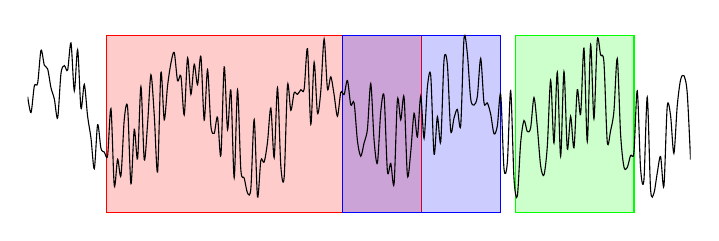
\begin{tikzpicture}[samples=200, domain=0:5*360]
			
				\draw[draw=red,fill=red,fill opacity=0.2] (1,0) rectangle ++(4,2.25);
				\draw[draw=blue,fill=blue,fill opacity=0.2] (4,0) rectangle ++(2,2.25);
				\draw[draw=green,fill=green,fill opacity=0.2] (6.2,0) rectangle ++(1.5,2.25);

        		\begin{axis}[
            		width=10cm, height=4cm,
            		enlarge x limits=false,
            		hide x axis,
            		hide y axis
        		]
        			\addplot [no markers, smooth] {sin(x)+rand*2};
        		\end{axis}
    		\end{tikzpicture}
			\caption{Event Detection in an audio track.}
			\label{fig:sounddetection}
		\end{figure}
		
	\end{frame}
	
	\begin{frame}{Datasets}
	
		Common datasets for Audio Segmentation and Sound Event Detection problems are:
		
		\begin{itemize}
			\item \textbf{TUT Sound Event Detection}: primarily consists of street recordings with traffic and other activity, with audio examples of \SI{2.56}{\second} and a total size of approximately \SI{1.5}{\hour}. It has six unique audio classes -- Brakes Squeaking, Car, Children, Large Vehicle, People Speaking, and People Walking;
			\item \textbf{Urban-SED}: purely synthetic dataset, with audio example of \SI{10}{\second} and a total size of about \SI{30}{\hour}. It has ten unique audio classes -- Air Conditioner, Car Horn, Children Playing, Dog Bark, Drilling, Engine Idling, Gun Shot, Jackhammer, Siren, and Street Music.
		\end{itemize}
		
		The first dataset is too small to train a Neural Network model and requires use of augmentation techniques (we used \textbf{SpecAugment}\footcite{park19e_interspeech}).
	\end{frame}
	
	\begin{frame}{Metrics}
	
		A popular toolbox for Polyphonic Sound Event Detection models evaluation is \textbf{SED Eval}\footcite{app6060162}.
	
		\begin{multicols}{2}
  			\begin{equation*}
    			\text{Precision} = \frac{\text{TP}}{\text{TP} + \text{FP}}
  			\end{equation*}\break
  			\begin{equation*}
    			\text{Recall} = \frac{\text{TP}}{\text{TP} + \text{FN}}
  			\end{equation*}
		\end{multicols}

		$$
			\text{F$_{1}$-score} = 2 \times \frac{\text{Precision} \times \text{Recall}}{\text{Precision} + \text{Recall}}
		$$
	\end{frame}

	%!TEX TS-program = pdflatex
%!TEX root = ../main.tex
%!TEX encoding = UTF-8 Unicode


\section[YOHO model]{YOHO model}

	\begin{frame}{YOHO model}
			
		Presented in 2021\cite{Venkatesh_2022}\dots
		
		\note{
			\dots			
		}		
		
	\end{frame}
	
	\begin{frame}{Input shape}
		\dots
		
		\note{
			\dots
		}
	\end{frame}
	
	
	\begin{frame}{Network Architecture}
		\dots
		
		\note{
			\dots
		}
	\end{frame}
	
	
	\begin{frame}{Output shape}
	
	\begin{figure}
			\centering
			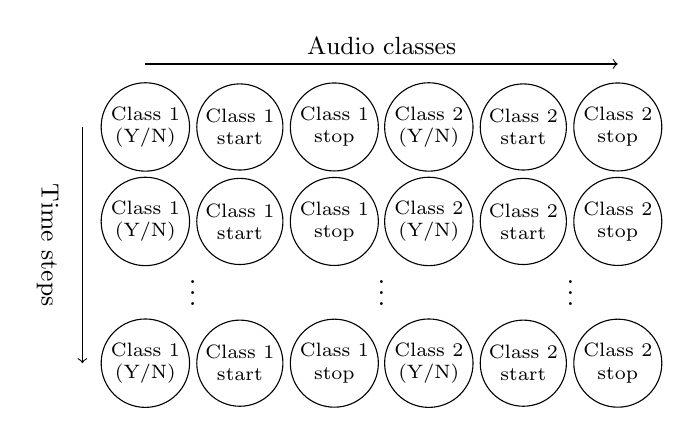
\begin{tikzpicture}[scale=.8]
			
				\draw [->,black] (1,6) -- node[midway,above]{\small Audio classes} (8.5,6);
				\draw [->,black] (0,5) -- node[midway,left,below=5pt,sloped]{\small Time steps} (0,1.25);
				
				\node[circle,draw,align=center,inner sep=0pt,text width=1cm,font = {\scriptsize}] at (1,5) {Class $1$\\(Y/N)};
				\node[circle,draw,align=center,inner sep=0pt,text width=1cm,font = {\scriptsize}] at (2.5,5) {Class $1$\\start};
				\node[circle,draw,align=center,inner sep=0pt,text width=1cm,font = {\scriptsize}] at (4,5) {Class $1$\\stop};

				\node[circle,draw,align=center,inner sep=0pt,text width=1cm,font = {\scriptsize}] at (5.5,5) {Class $2$\\(Y/N)};
				\node[circle,draw,align=center,inner sep=0pt,text width=1cm,font = {\scriptsize}] at (7,5) {Class $2$\\start};
				\node[circle,draw,align=center,inner sep=0pt,text width=1cm,font = {\scriptsize}] at (8.5,5) {Class $2$\\stop};


				\node[circle,draw,align=center,inner sep=0pt,text width=1cm,font = {\scriptsize}] at (1,3.5) {Class $1$\\(Y/N)};
				\node[circle,draw,align=center,inner sep=0pt,text width=1cm,font = {\scriptsize}] at (2.5,3.5) {Class $1$\\start};
				\node[circle,draw,align=center,inner sep=0pt,text width=1cm,font = {\scriptsize}] at (4,3.5) {Class $1$\\stop};

				\node[circle,draw,align=center,inner sep=0pt,text width=1cm,font = {\scriptsize}] at (5.5,3.5) {Class $2$\\(Y/N)};
				\node[circle,draw,align=center,inner sep=0pt,text width=1cm,font = {\scriptsize}] at (7,3.5) {Class $2$\\start};
				\node[circle,draw,align=center,inner sep=0pt,text width=1cm,font = {\scriptsize}] at (8.5,3.5) {Class $2$\\stop};

				\node[align=center] at (1.75,2.5) {$\vdots$};
				\node[align=center] at (4.75,2.5) {$\vdots$};
				\node[align=center] at (7.75,2.5) {$\vdots$};

				\node[circle,draw,align=center,inner sep=0pt,text width=1cm,font = {\scriptsize}] at (1,1.25) {Class $1$\\(Y/N)};
				\node[circle,draw,align=center,inner sep=0pt,text width=1cm,font = {\scriptsize}] at (2.5,1.25) {Class $1$\\start};
				\node[circle,draw,align=center,inner sep=0pt,text width=1cm,font = {\scriptsize}] at (4,1.25) {Class $1$\\stop};

				\node[circle,draw,align=center,inner sep=0pt,text width=1cm,font = {\scriptsize}] at (5.5,1.25) {Class $2$\\(Y/N)};
				\node[circle,draw,align=center,inner sep=0pt,text width=1cm,font = {\scriptsize}] at (7,1.25) {Class $2$\\start};
				\node[circle,draw,align=center,inner sep=0pt,text width=1cm,font = {\scriptsize}] at (8.5,1.25) {Class $2$\\stop};

			\end{tikzpicture}
			\caption{The YOHO output shape.}
			\label{fig:YOHOoutput}
		\end{figure}
		
	\end{frame}
	

	\begin{frame}{Loss Function}
		\begin{equation*}
			\mathcal{L}_{c}(\hat{y},y) = \begin{cases}
			(\hat{y}_1-y_1)^2+\\(\hat{y}_2-y_2)^2+(\hat{y}_3-y_3)^2 &\text{if $y_{1} = 1$}\\
			(\hat{y}_1-y_1)^2, &\text{if $y_1 = 0$}
			\end{cases}
		\end{equation*}
		
		where $y$ and $\hat{y}$ are the ground-truth and predictions respectively. $y_1 = 1$ if the acoustic class is present and $y_1 = 0$ if the class is absent. $y_2$ and $y_3$, which are the start and endpoints for each acoustic class are considered only if $y = 1$.
		In other words, $(\hat{y}_1-y_1)^2$ corresponds to \textbf{the classification loss} and $(\hat{y}_2-y_2)^2+(\hat{y}_3-y_3)^2$ corresponds to \textbf{the regression loss}.
		\note{
			\dots
		}
	\end{frame}
	
	\begin{frame}{Other Details}
		\dots
		
		\note{
			\dots
		}
	\end{frame}


\section[Implementation details]{Implementation details}	

	\begin{frame}{Implementation details}
		\dots
		
		\note{
			\dots			
		}		
		
	\end{frame}

	\begin{frame}{Problems}
		\dots
		
		\note{
			\dots			
		}		
		
	\end{frame}


	%!TEX TS-program = pdflatex
%!TEX root = ../main.tex
%!TEX encoding = UTF-8 Unicode


\section[Conclusions]{Conclusions}
	
	\begin{frame}{Project workflow}
		\begin{figure}
			\centering
			\begin{tikzpicture}
   				\node[anchor=south west,inner sep=0] at (0,0) {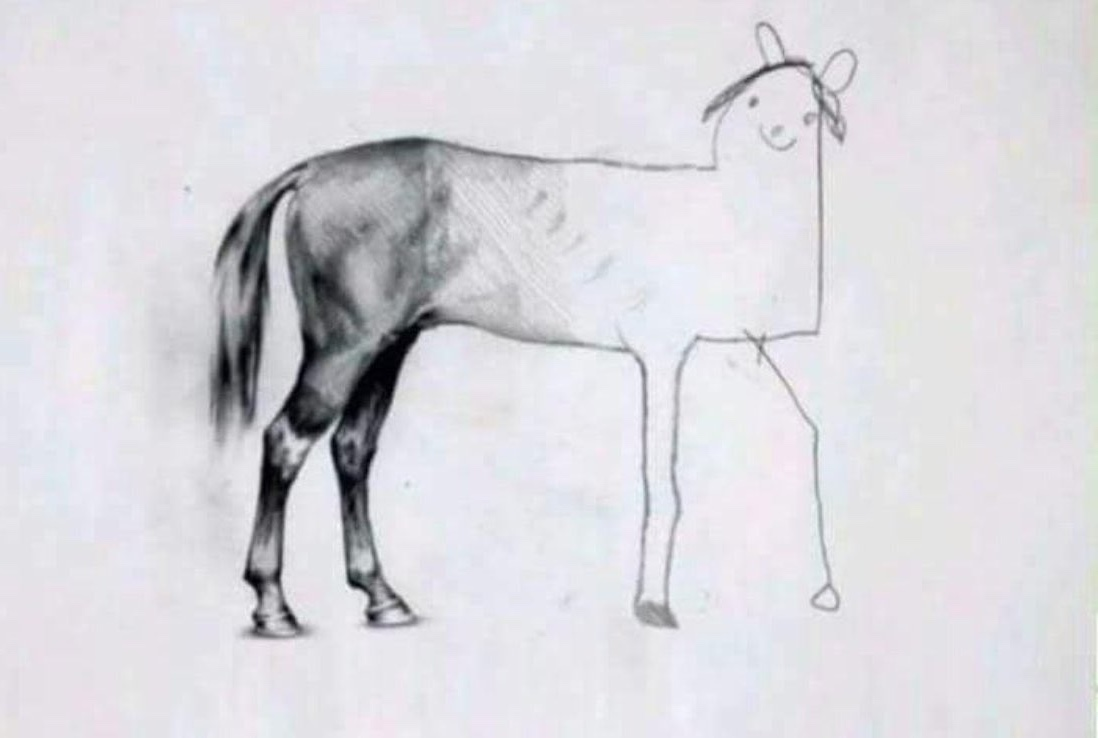
\includegraphics[width=.6\textwidth]{./images/horse.jpg}};
				
				\node[draw,align=center,fill=white,inner sep=1pt,font = {\scriptsize}] at (1.75,.2) {First\\month};
    	
				\draw[thick] (3.25,0) -- (3.25,5.65);

				\node[draw,align=center,fill=white,inner sep=1pt,font = {\scriptsize}] at (3.8,.2) {Second\\month};
    		
				\draw[thick] (4.35,0) -- (4.35,5.65);

				\node[draw,align=center,fill=white,inner sep=1pt,font = {\scriptsize}] at (4.9,.2) {Third\\month};

    			\draw[thick] (5.5,0) -- (5.5,5.65);
			
				\node[draw,align=center,fill=white,inner sep=1pt,font = {\scriptsize}] at (7,.2) {One week\\to the exam};

			\end{tikzpicture}

			\caption{The roadmap of our journey.}
			\label{fig:roadmap}
		\end{figure}
	\end{frame}
	
	\begin{frame}{Our 2 cents}
	Our contribution
	\end{frame}

	\begin{frame}{Conclusions}
	
		But, after all\dots
		
		\begin{quote}
        	It's all about the journey, not the destination.
      	\end{quote}
	
		Thank you for your attention.
     
	\end{frame}

\end{document}